%!TEX root = paper.tex
%%%%%%%%%%%%%%%%%%%%%%%%%%%%%%%%%%%%%%%%%%%%%%%%%%%%%%%%%%%%%%%%%%%%%%%%%%%%%%%%
\section{Introduction}
\label{sec:introduction}

A common trend in online video game \gls{QoE} assessments (for both multiplayer and cloud games) is the apparent obliviousness of such studies to the inner workings of video games. This especially means understanding the main game loop with its tick rates as well as mechanics and implications surrounding the framerate. The diversity of games and their accompanying gameplay mechanics also makes it difficult to transfer any findings from one game to another. Yet, in order to conduct proper measurements, it is essential to understand these mechanics, resulting in a better, quantitative classification of games based on game \textit{properties} rather than opaque and less effective \textit{categories} like \gls{FPS} or \gls{RPG}, and thus a basis for an objective quality assessment model. To facilitate this, this work investigates gaming properties, especially a game's framerate and tickrate, on the basis of the ``\gls{E2E} lag'' using a model and queuing simulation. Initial results visualize that the influence of the framerate and tickrate on the \gls{E2E} lag, and therefore also on the subjective quality of the game, is much larger than expected. This means that these two parameters need to be tightly controlled in subjective quality assessment studies.


\begin{figure}[!t]
	\centering
	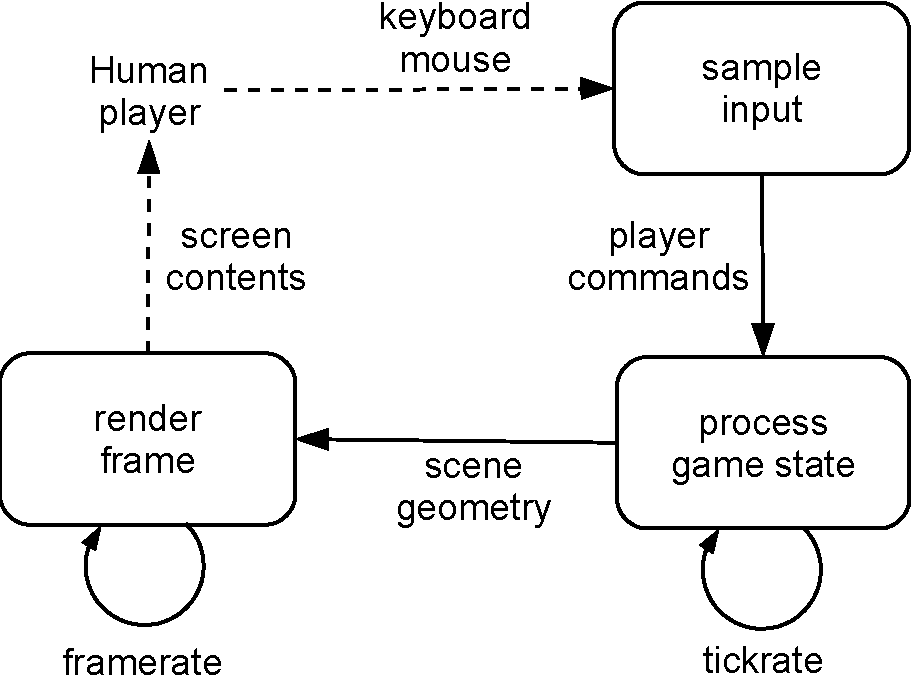
\includegraphics[width=0.8\columnwidth]{../../../models/game_loop.pdf}
	\caption{Basic model of a continuous main video game loop.}
	\label{fig:gameloop1}
\end{figure}

\begin{table}[!t]
\caption{Tickrates in competitive and popular video games that are either known, speculated upon, or derived by counting update and command messages. Data was collected from various sources and should be taken as-is.}
% \hoss{Welche rel. bzw. unreliable sources? Gibt es auch typische framerates dazu?}
% fm: inoffizielle, nicht-wissenschaftliche quellen, da diese werte normalerweise nicht durch den entwickler veröffentlicht werden; für framerates gibt es keine werte, da diese normalerweise unlocked laufen (zumindest für pc, bei konsolen für alle entweder 30 oder 60), ist eigentlich zu komplex um an der stelle darauf einzugehen
\label{tbl:tickrates}
	\centering
	\begin{tabu}{X[0.45]X}
		\toprule
		\textbf{Video Game} & \textbf{Tickrate} \\
		\midrule
		CS: GO & Configurable \SI{64}{\hertz}/\SI{128}{\hertz} \\
		Battlefield 4 & \SI{30}{\hertz}; \SI{10}{\hertz} for state outside of close proximity to player; \SI{60}{\hertz}/\SI{120}{\hertz} on test servers. \\
		Minecraft & max. \SI{20}{\hertz} \\
		League of Legends & \SI{30}{\hertz} (estimated) \\
		Dota 2 & \SI{30}{\hertz} \\
		StarCraft II & supposedly either \SI{16}{\hertz} or \SI{32}{\hertz} \\
		Eve Online & \SI{1}{\hertz} \\
		Project Cars & \SI{600}{\hertz} (Physics), \SI{250}{\hertz} (Input) \\ %https://twitter.com/projectcarsgame/status/551340759858040833
		\bottomrule
	\end{tabu}
\end{table}

\begin{figure*}[!t]
  \centering
  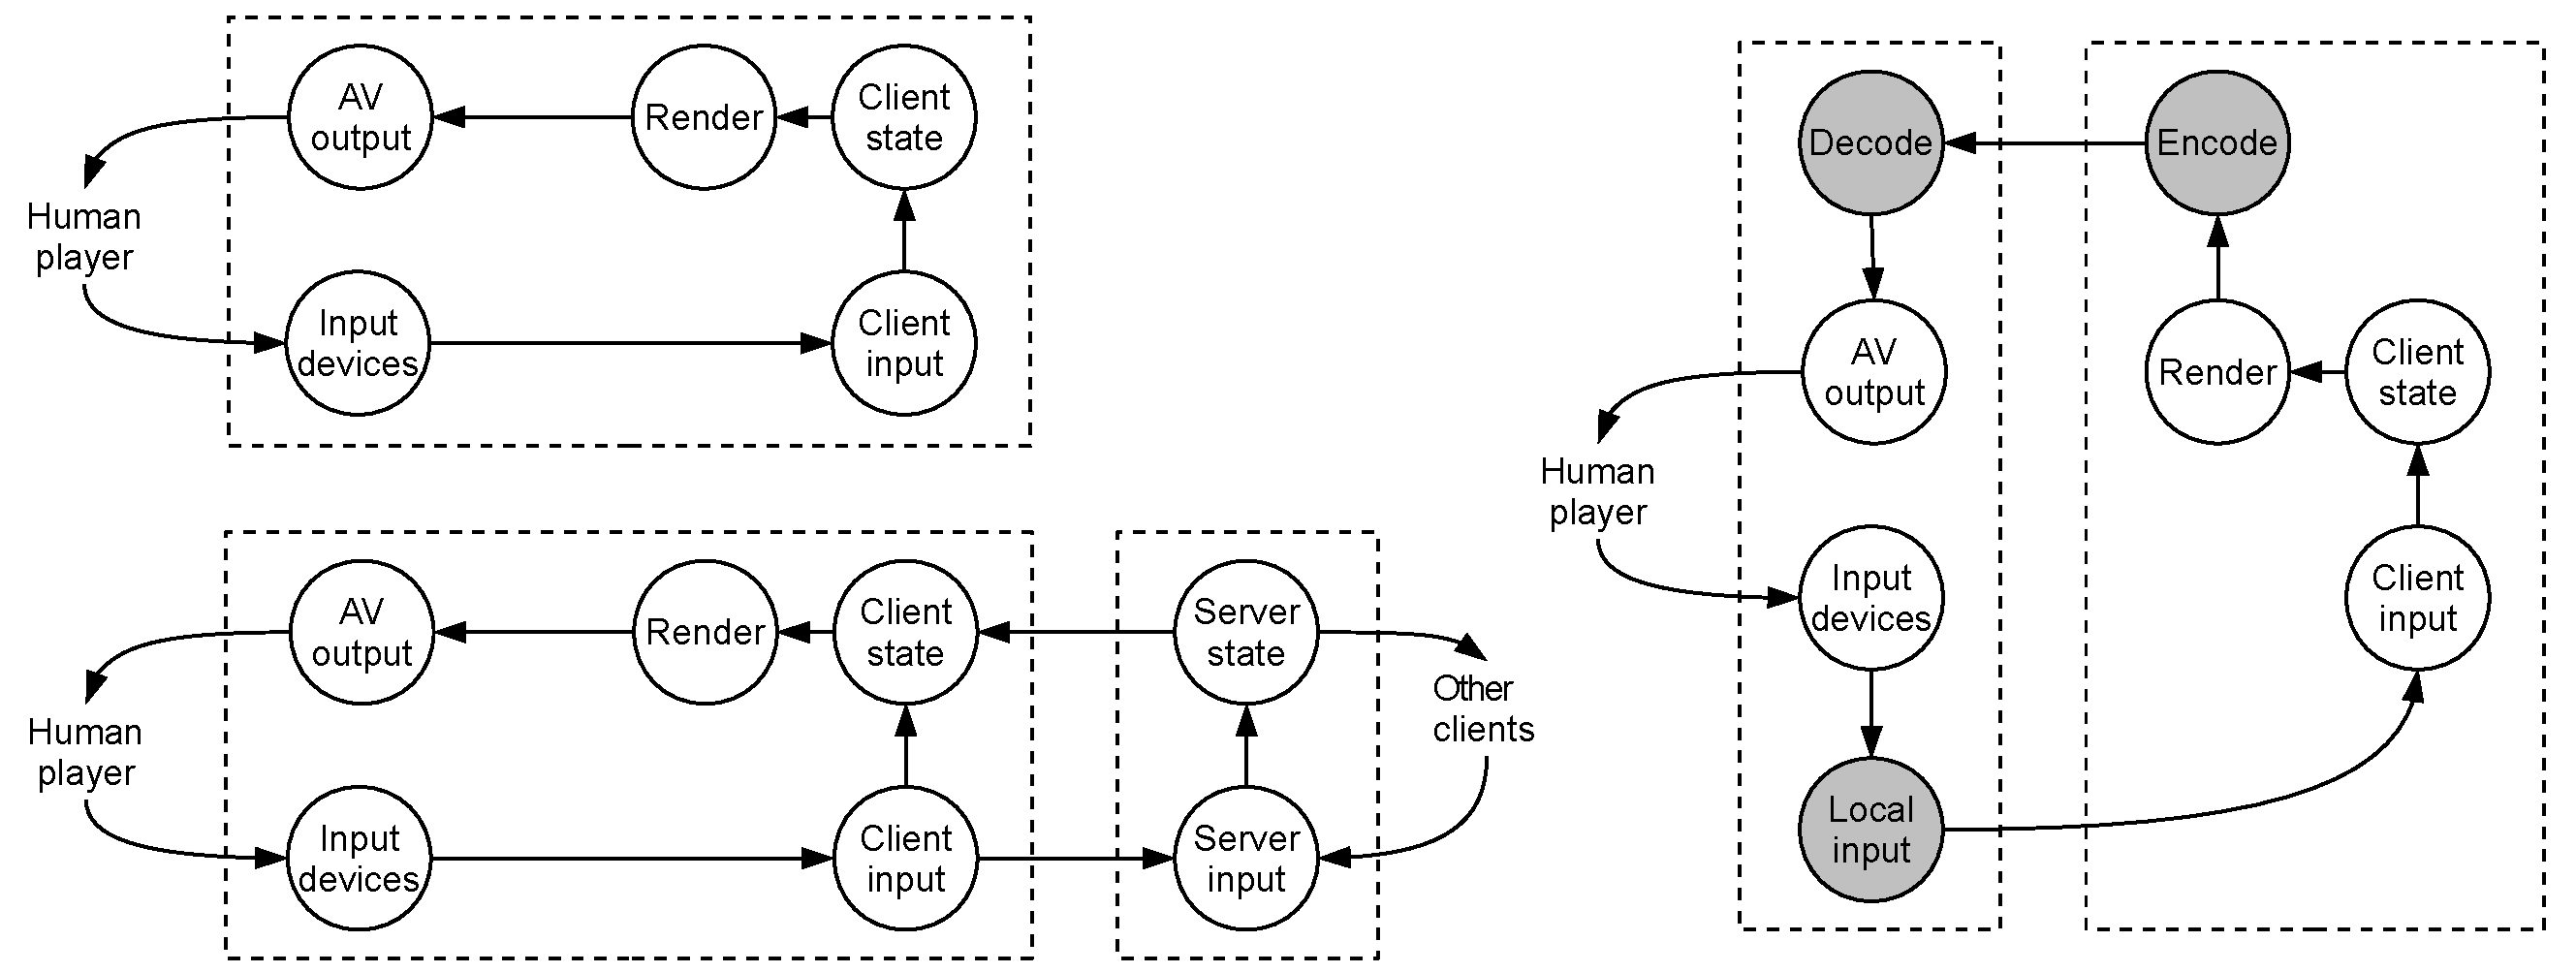
\includegraphics[width=0.9\textwidth]{../../../models/component_interaction_full.pdf}
  \caption{Interactions between components in different video game models. \textit{(a)} Single-player, \textit{(b)} online, \textit{(c)} cloud game.}
  \label{fig:component-models}
\end{figure*}

\begin{figure}[!t]
    \centering
    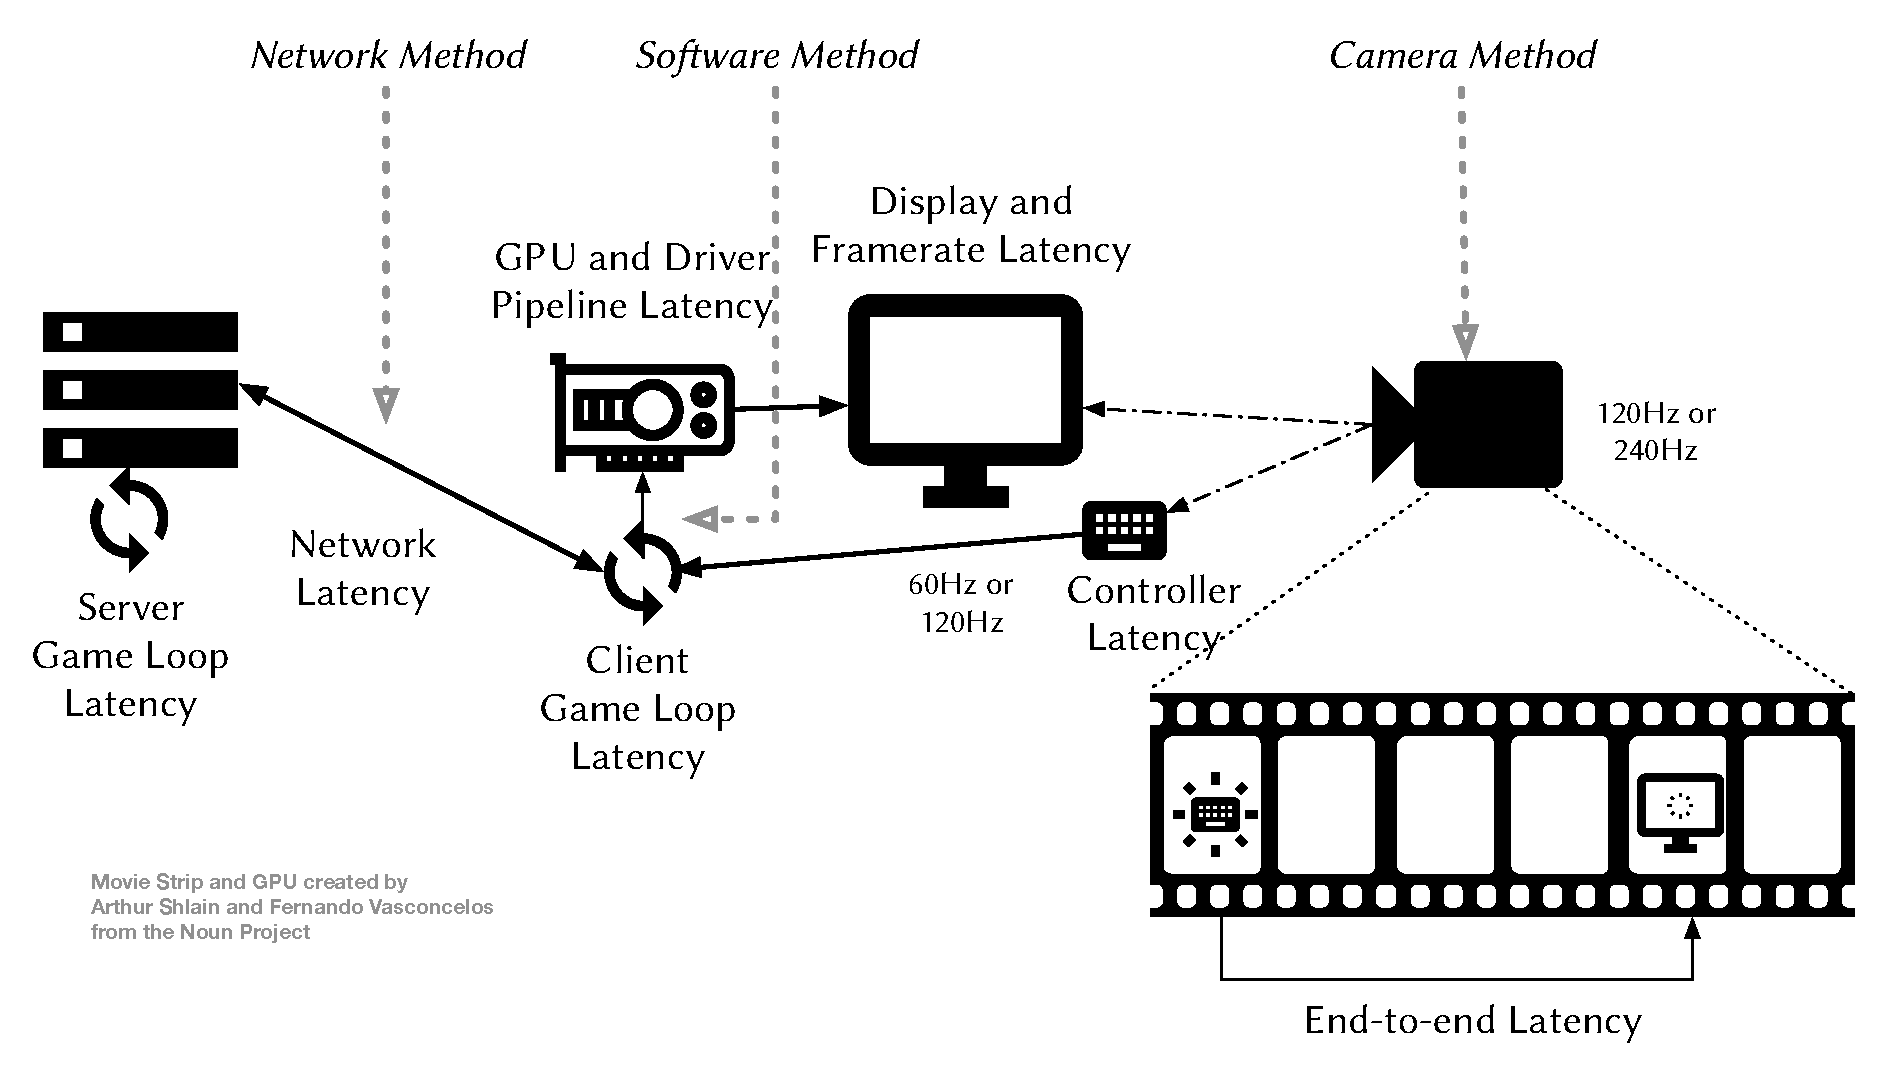
\includegraphics[width=1.0\columnwidth]{../../../models/e2e-lag.pdf}
    \caption{Location of three measurement approaches to capture end-to-end lag in an online video game.}
\label{fig:measurement-methods}
\end{figure}



\begin{table}[!t]
\caption{Notation used in the model. Random variables are denoted by capital letters $X$, and constants by small letters $x$.}
\label{tab:notation}
	\centering
	\begin{tabu}{lX[1,l]X[1,l]}
	\toprule
	\textbf{Symbol} & \textbf{Description} & \textbf{Simulation} \\
	\midrule
	$D$ & network delay between game client and server & $D \sim TNorm(\mu_D;\sigma_D)$, $\mu_D = \SI{20}{\milli\second}$; $\sigma_D = \SI{5}{\milli\second}$\\
	$P$ & game server processing time & $P \sim TNorm(\mu_P;\sigma_P)$, $ \mu_P = \SI{3}{\milli\second}; \sigma_P = \SI{0.1}{\milli\second}$\\
	$T$ & end-to-end lag & key performance measure \\
	$U$ & (inter arrival) time between user inputs & $U \sim Exp(\lambda)$; $\lambda = \SI{50}{\milli\second}$\\
	\midrule
	$c$ & command rate & $c=g$ \\
	$c^{-1}$ & interval to gather input events before sending & \\
	$d$ & decode delay & \SI{5}{\milli\second} \\
	$e$ & encode delay & \SI{15}{\milli\second} \\
	$f$ & framerate & $f \in \SIrange{10}{200}{\hertz}$ \\
	$f^{-1}$ & frame duration & $f^{-1} \in \SIrange{5}{100}{\milli\second}$ \\
	$g$ & game tickrate & $g \in \SIrange{10}{200}{\hertz}$ \\
	$g^{-1}$ & game tick duration & $g^{-1} \in \SIrange{5}{100}{\milli\second}$ \\
	\bottomrule
	\end{tabu}
\end{table}



\begin{figure}[!t]
	\centering
	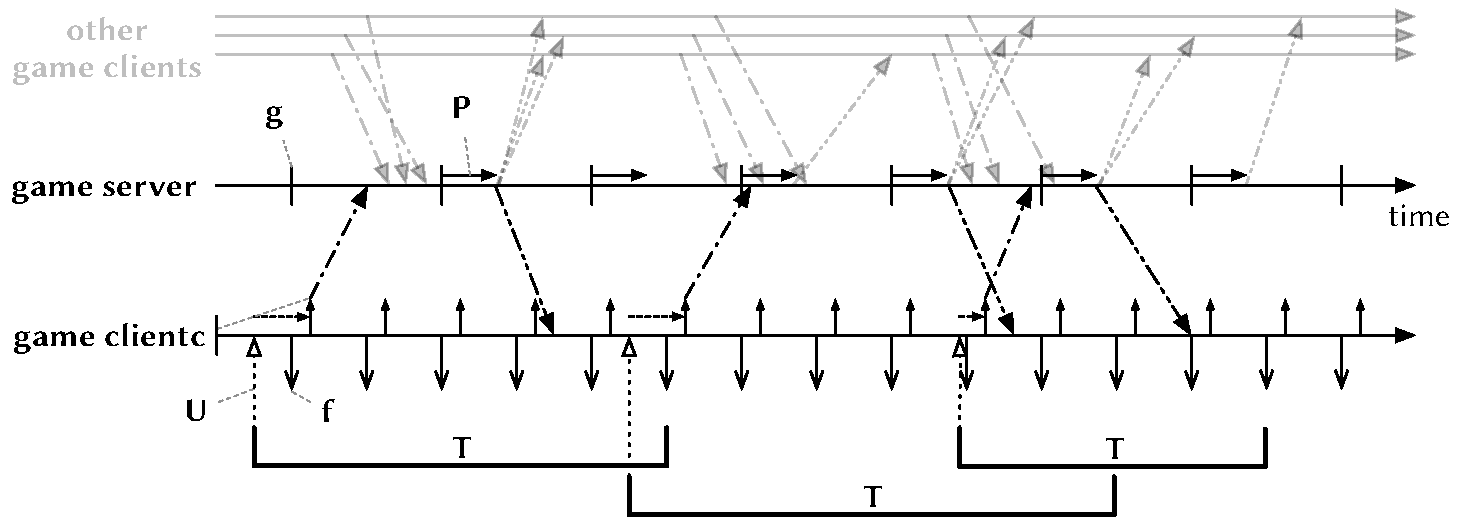
\includegraphics[width=1.0\columnwidth]{../../../models/tickrate-timeseries-notation.pdf}
	\caption{Exemplary flow of events in an online client-server game, and resulting end-to-end lag with the notation of Tab.~\ref{tab:notation}.
	% \hoss{Notation aus Tabelle ~\ref{tab:notation} waere gut im Bild. }
	} %Delay values are given for a framerate of \SI{60}{\hertz} and a server tickrate of \SI{30}{\hertz}, the network latency will only show minor variations.}
\label{fig:tickrate-timeseries}
\end{figure}


\begin{figure}[!t]
	\centering
	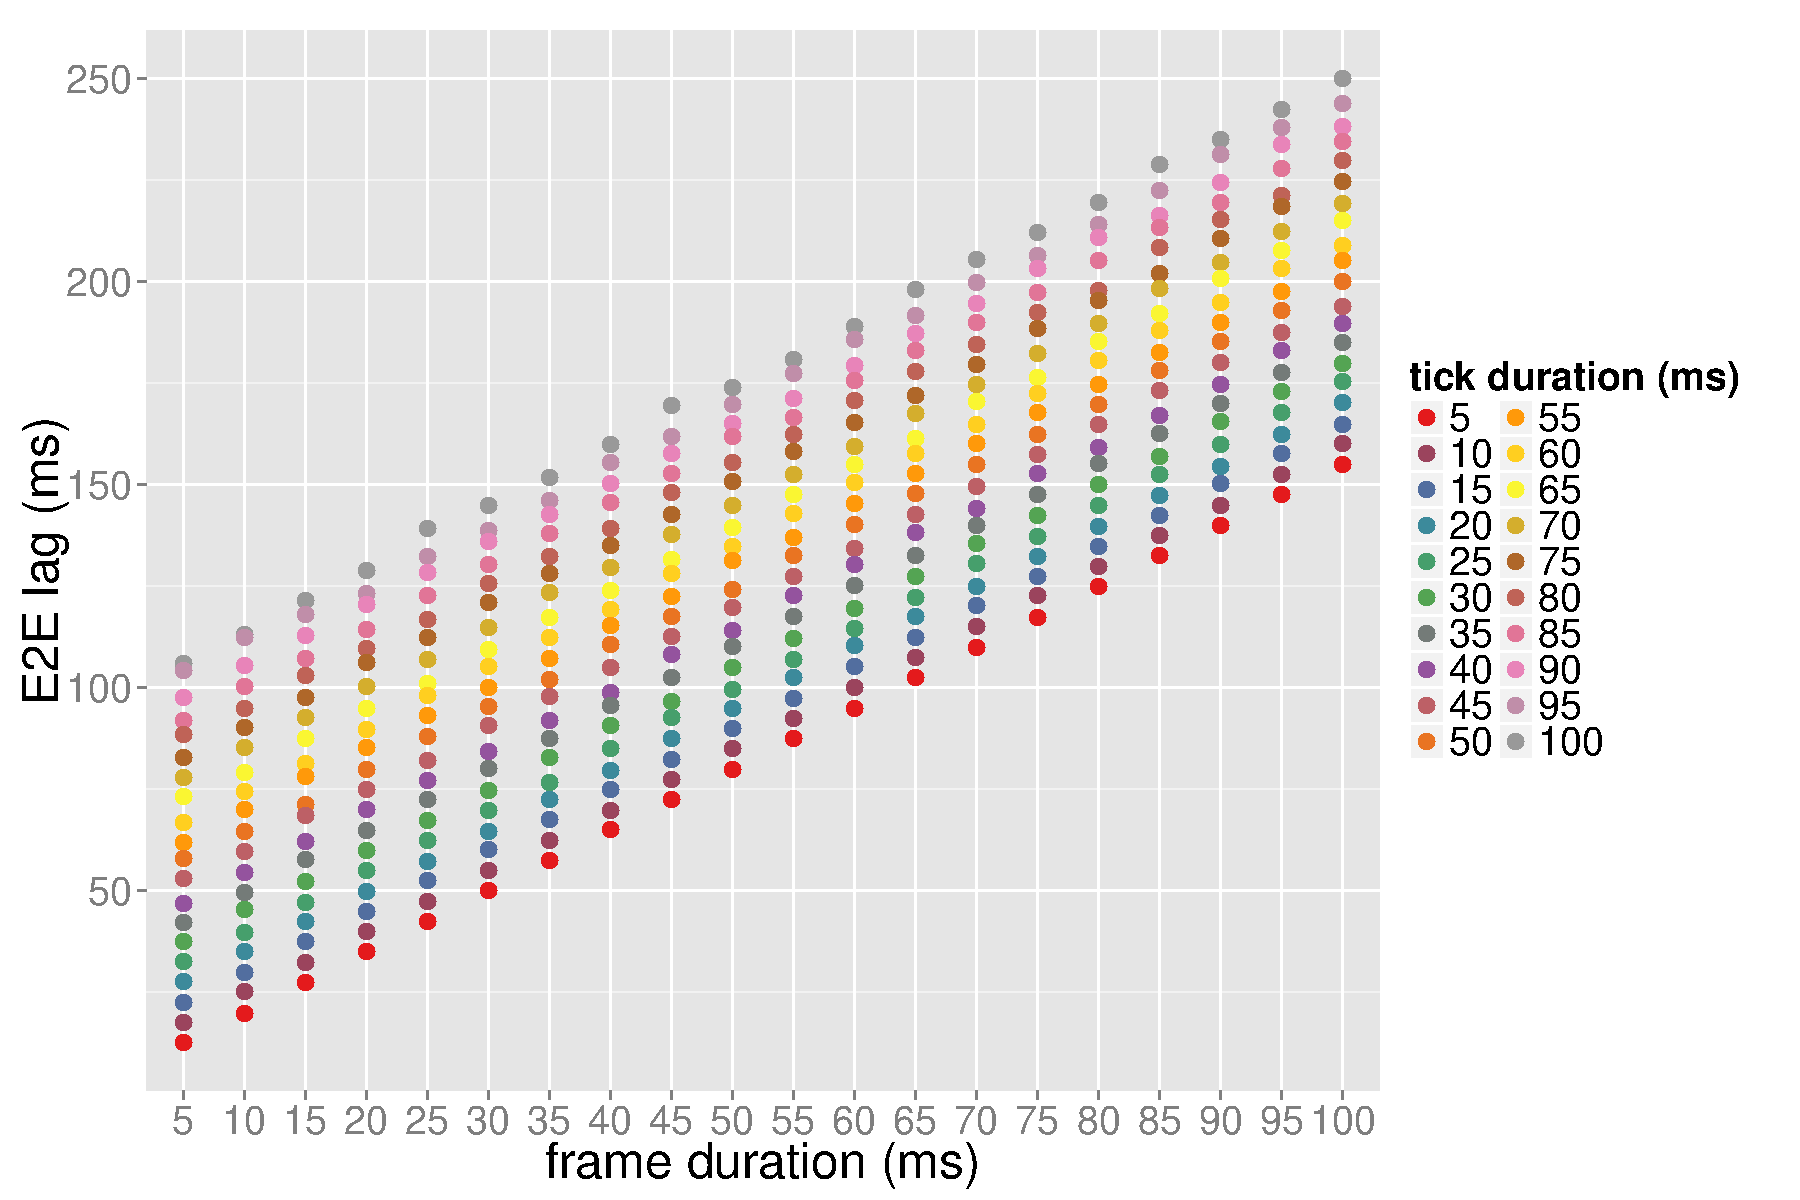
\includegraphics[width=1.0\columnwidth]{../../../simulation/visualization/nwless-onlinegame-1000rounds.pdf}
	\caption{Median end-to-end lag under various frame and tick durations for a locally-running game. Lower lag values are achieved at lower frame and tick durations.}
\label{fig:nwless-scatter}
\end{figure}


\begin{figure}[!t]
	% TODO: adjust the bounding box of the 3dbar plot, instead of playing with fire (aka \vspace)
	\centering
	\vspace{-6mm}
	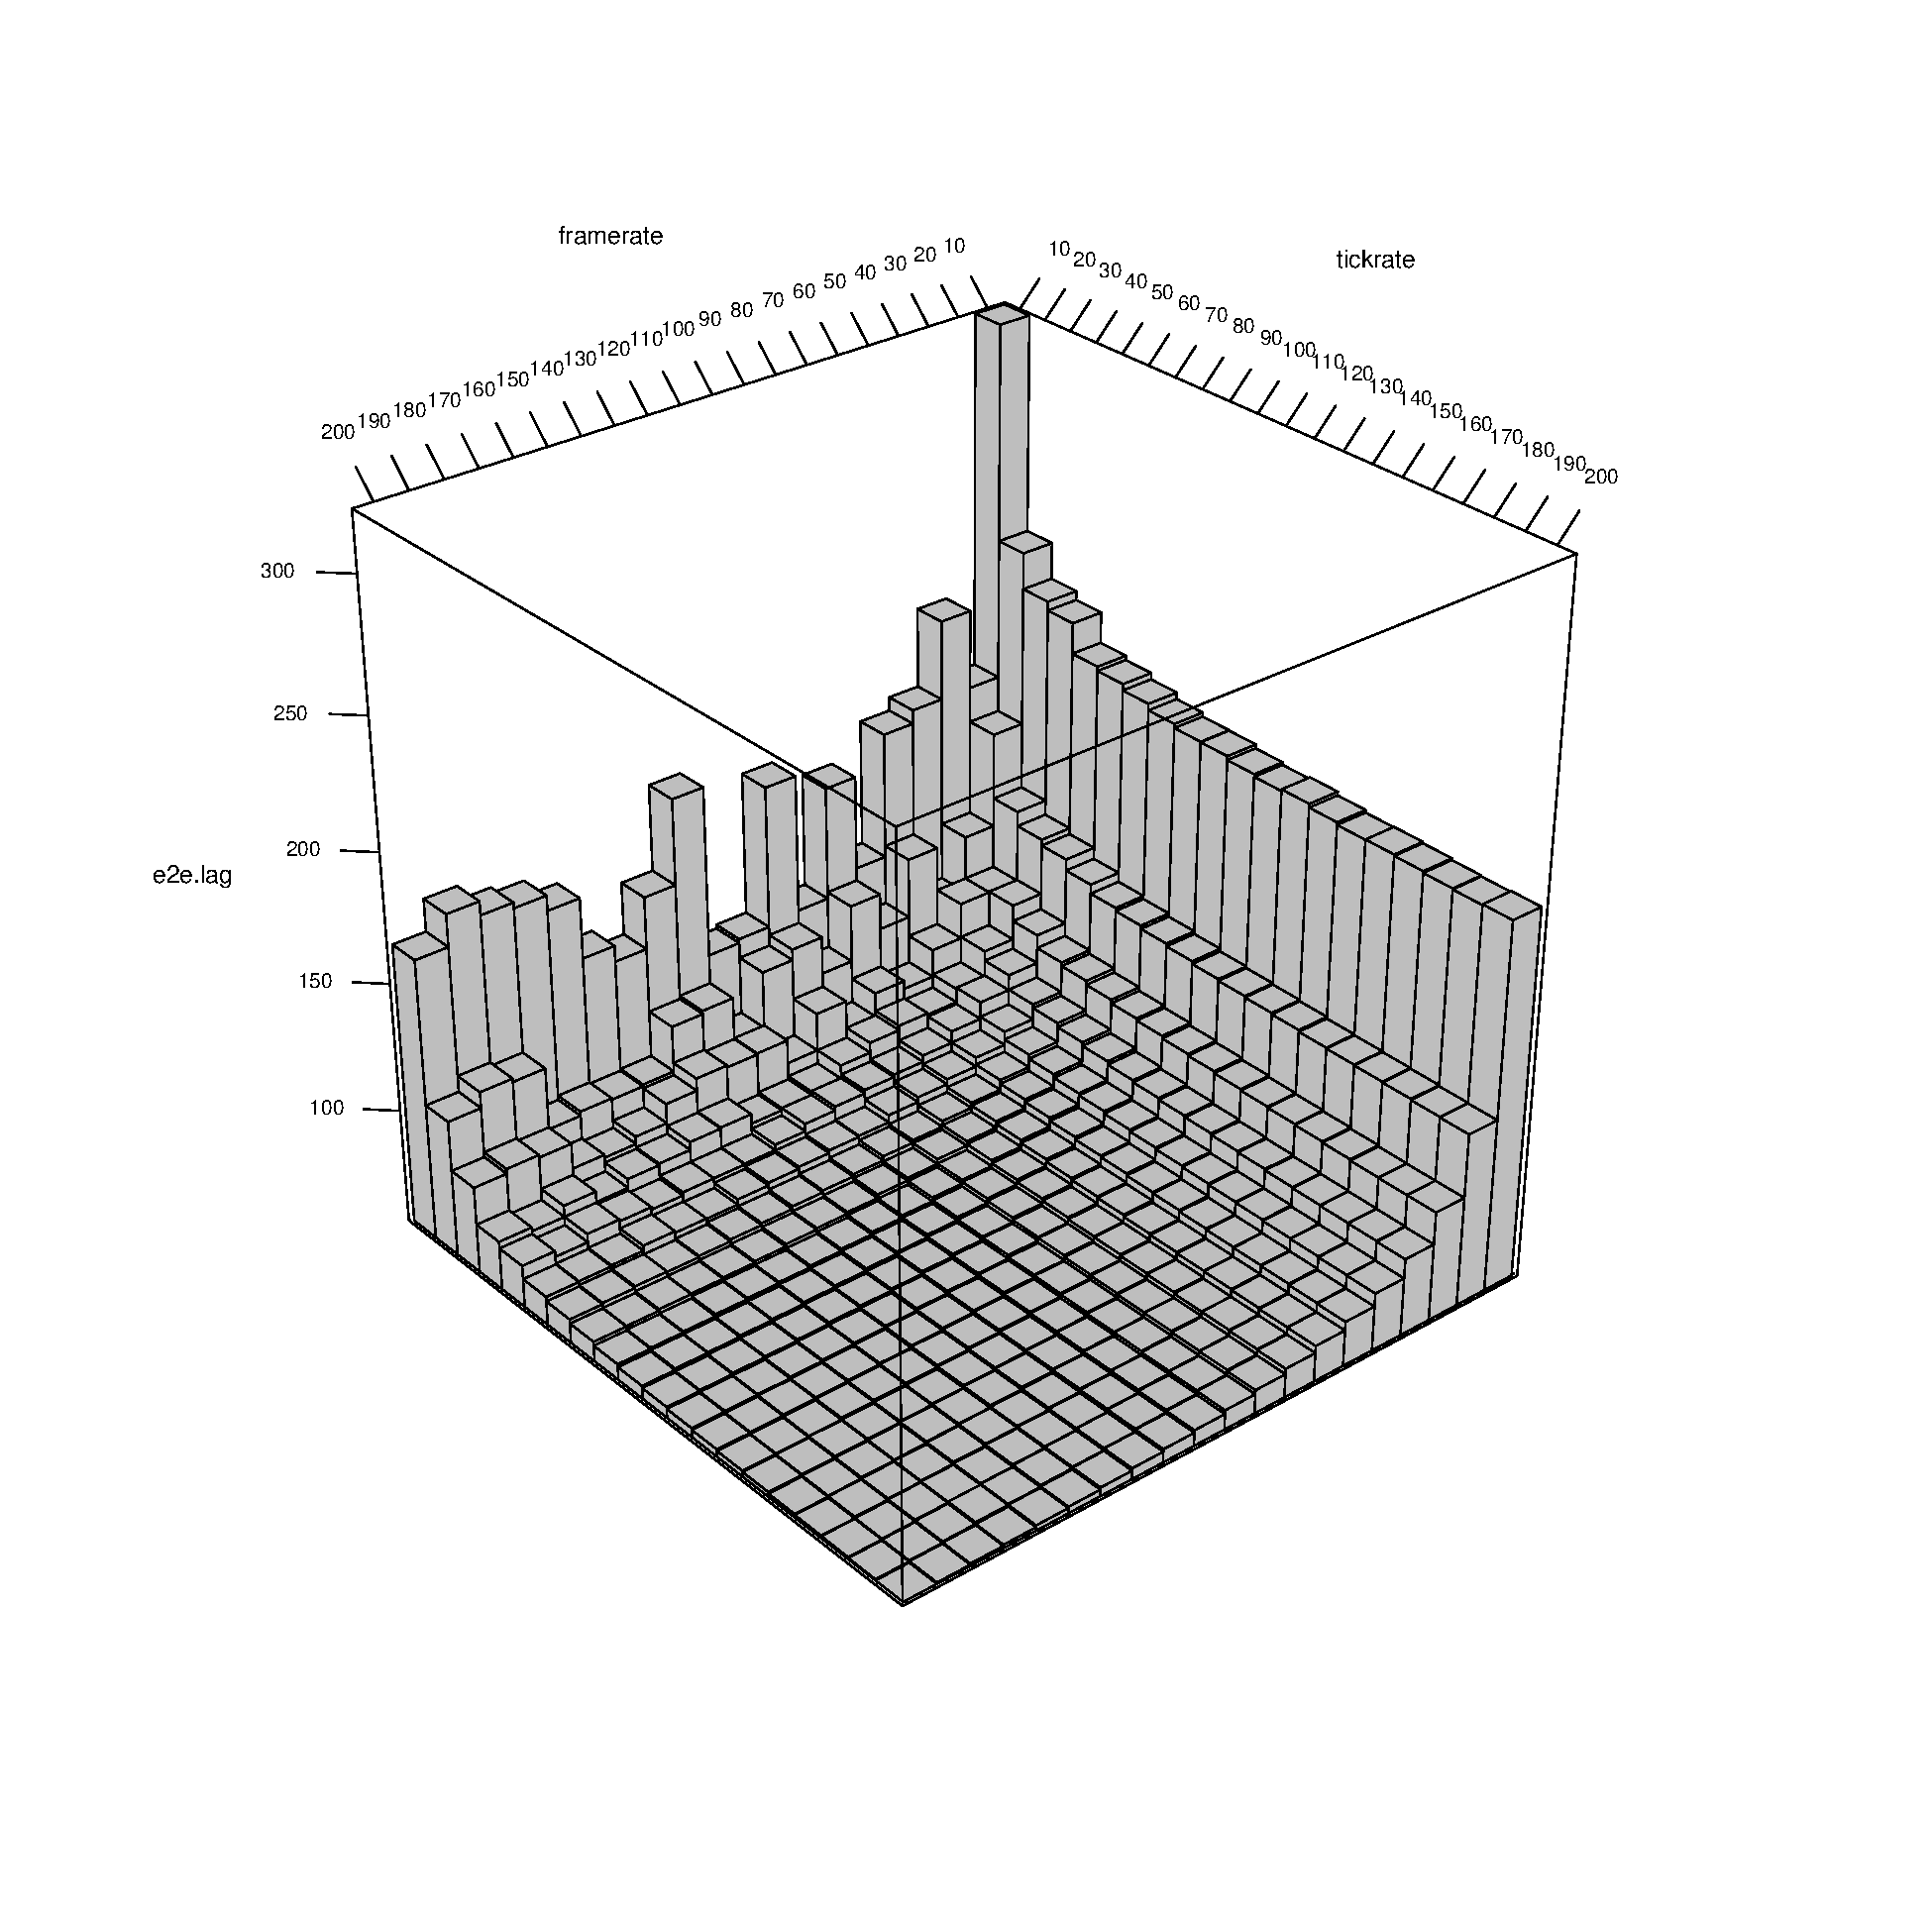
\includegraphics[width=1.0\columnwidth]{../../../simulation/visualization/e2e-lag-3dbars.pdf}
	\vspace{-15mm}
	\caption{Influence of client framerate and server tickrate on the median end-to-end lag in the online game scenario. For high rates $f$, $g$, the lag approaches $2\mu_D+\mu_P=\SI{43}{\milli\second}$.}
	% TODO: \hoss{Kann man hier einen stacked bar plot bauen, bei dem man den Networking Anteil sieht? Das wuerde die Aussage gut unterstuetzen.}
	% TODO: nicht rechtzeitig für submission deadline, aber für eine nächste version
\label{fig:3dbars-framerate-tickrate-lag}
\end{figure}

